% Eriq Augustine
%
% Cal Poly Thesis
%
% based on UC Thesis format
%
% modified by Mark Barry 2/07.
%

\documentclass[12pt]{ucthesis}

\usepackage{url}
\usepackage{hyperref}
\usepackage{graphicx}
\usepackage{amssymb}
\usepackage{amsmath}
\usepackage[letterpaper]{geometry}
\usepackage[overload]{textcase}
\usepackage{color}
\usepackage[nonumberlist,toc]{glossaries}
\usepackage{wrapfig}

\definecolor{orange}{rgb}{1,0.5,0}
\definecolor{blue}{rgb}{0.1,0.1,0.8}
\definecolor{green}{rgb}{0,0.5,0}
\definecolor{red}{rgb}{0.8,0,0}
\definecolor{bad}{rgb}{0.8,0,0.8}

\makeindex
\makeglossaries

\bibliographystyle{abbrv}

\setlength{\parindent}{0.25in} \setlength{\parskip}{6pt}
\geometry{verbose,nohead,tmargin=1.25in,bmargin=1in,lmargin=1.5in,rmargin=1.3in}
\setcounter{tocdepth}{2}

% Different font in captions (single-spaced, bold) ------------
\newcommand{\captionfonts}{\small\bf\ssp}

\makeatletter  % Allow the use of @ in command names
\long\def\@makecaption#1#2{%
  \vskip\abovecaptionskip
  \sbox\@tempboxa{{\captionfonts #1: #2}}%
  \ifdim \wd\@tempboxa >\hsize
    {\captionfonts #1: #2\par}
  \else
    \hbox to\hsize{\hfil\box\@tempboxa\hfil}%
  \fi
  \vskip\belowcaptionskip}
\makeatother   % Cancel the effect of \makeatletter
% ---------------------------------------

\begin{document}

% Declarations for Front Matter

% Update fields below!
\title{SPOONS: Netflix Outage Detection Using Microtext Classification}
\author{Eriq Augustine}
\degreemonth{March} \degreeyear{2012} \degree{Master of Science}
\defensemonth{March} \defenseyear{2012}
\numberofmembers{3} \chair{Alex Dekhtyar, Ph.D.} \othermemberA{Clint Staley, Ph.D.} \othermemberB{Franz Kurfess, Ph.D.} \othermemberC{Foaad Khosmood, Ph.D.} \field{Computer Science} \campus{San Luis Obispo}
\copyrightyears{seven}

\maketitle

\begin{frontmatter}

% Custom made for Cal Poly (by Mark Barry, modified by Andrew Tsui).
\copyrightpage

% Custom made for Cal Poly (by Andrew Tsui).
\committeemembershippage

\begin{abstract}

Every week there are over a billion new posts to Twitter services and many of
those messages contain feedback to companies about their services. One company
that has recognized this unused source of information is Netflix. That is why
Netflix initiated the development of a system that will let them respond to the
millions of Twitter and Netflix users that are acting as sensors and reporting all types of user
visible outages. This system will enhance the feedback loop between Netflix and
its customers by increasing the amount of customer feedback that is being
received by Netflix and reducing the time it takes for Netflix to receive the
reports and respond to them.

The goal of the SPOONS (Swift Perceptions of Online Negative Situations) system
is to use Twitter posts to determine when Netflix users are reporting a problem
with any of the Netflix services. This work covers the architecture SPOONS system and framework
as well as outage detection using tweet classification.

\end{abstract}

\begin{acknowledgements}

Thanks Alex, thanks Netflix (Kevin).
Negative thanks to Farscape.

\end{acknowledgements}

\tableofcontents

\listoftables

\listoffigures

\end{frontmatter}

\pagestyle{plain}

\renewcommand{\baselinestretch}{1.66}

% ------------- Main chapters here --------------------

\chapter{Introduction}
\label{introduction}

\section{General Problem: Swift Perception Of Online Negative Situations}
\label{general-problem}

Twitter is an immensely popular micro-blogging service. According to Twitter,
approximately one billion micro-posts, \emph{tweets}, were being poster per week as of March 14th 2011\cite{TwitterBlog}.
Because of the low time and effort cost of tweeting, only a few seconds from a smart phone,
Users of Twitter post tweets about almost every aspect of their daily lives.
Because of this large stream of information, Twitter makes an excellent source of information for
data miners. Already, researchers have been using Twitter to attempt to track and model
disease outbreaks\cite{DetectingInfluenza}, earthquakes\cite{Earthquakes}, and the
stock market\cite{StockMarket}.

Netflix saw the power in this data source as a potential for detecting service outages that
is orthogonal to their current outage detection methods. Currently, Netflix utilizes four
different methods for detecting outages:

\paragraph{Internal Monitoring Systems}
Like any sizable service providing company, Netflix utilizes many different internal monitoring
systems to detect service outages. However, there are some class of problems that are difficult to solve
with internal monitoring. These problems include broken encodes of video files or a problem on a third-party delivery
platform such as Roku or AppleTV. These problems are obvious to an end user, but very difficult to detect internally.
In addition, the internal monitoring systems share the same infrastructure as the service providing system. Therefore,
a problem in the infrastructre can cause both systems to go down at the same time.

\paragraph{External Monitoring Systems}
Netflix contracts with external services that can periodically probe its systems to try and detect problems.
However, this model too has problems. There are many problems that cannot be seen from an external probe.
Also, if this system probes too often then it is taking compute time away from the servers that are trying to deliver
content to end users.

\paragraph{Customer Service}
Calls to customer service are a very straight-forward way to detect outages.
Unfortunatley, this method is very slow and inconsistent. It takes a lot of frustration to get a user to
lookup a phone number and complain.

\paragraph{Manual Twitter Observation}
Manual observation shows that there is usually a response on Twitter when Netflix suffers a service
outage. Image~\ref{fig:tweetEx} shows some tweets that occured during a disruption of Netflix's serice to
the Nintendo Wii. However without any infrastructure, Twitter observation is slow and inconsistent.
It is also very time consuming to have someone constantly watching Twitter for signs of an outage.

Given all these deficiencies Netflix wanted a monitoring system that is seperate from their infrastructure,
fast, and does not require any human intervention\cite{kevin}.

% TODO(eriq): get a better tweet picture
\begin{figure}
   \begin{center}
      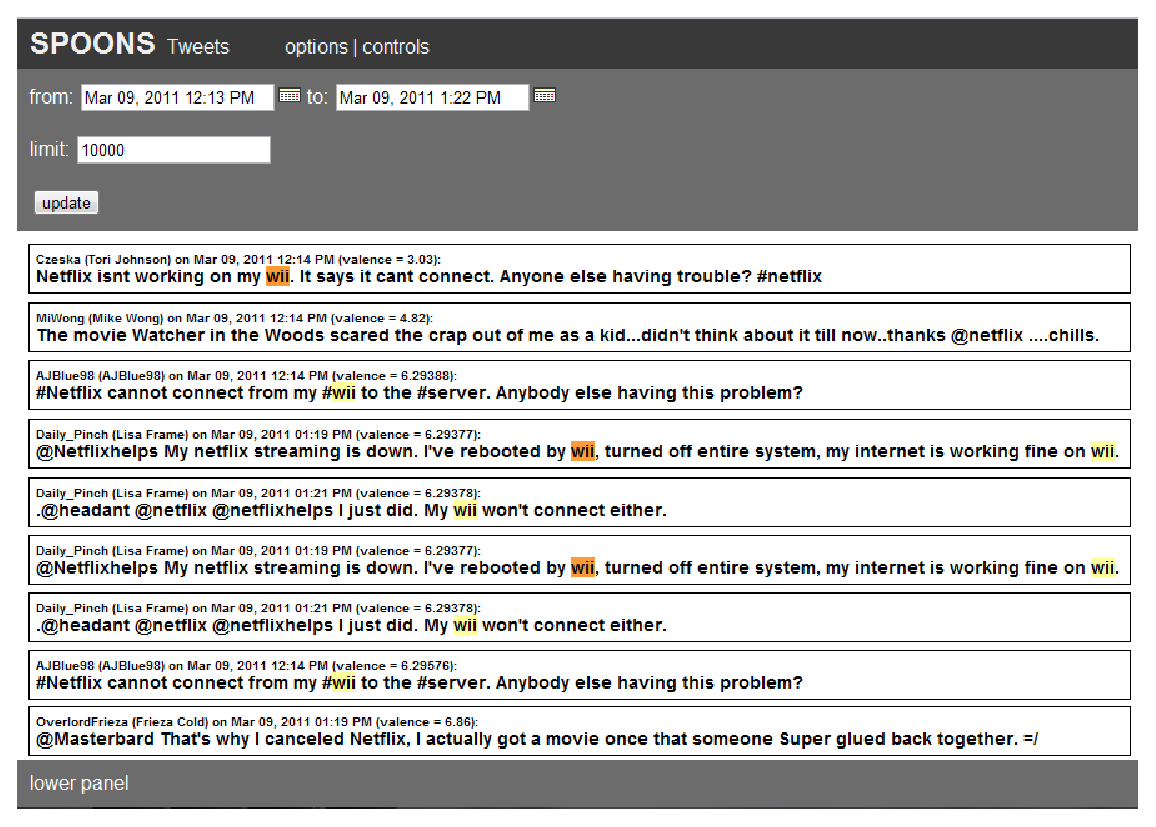
\includegraphics[width=140mm]{images/tweetexample.eps}
      \captionfonts
      \caption[Outage Tweets Example]{Tweets posted on March 9, 2011 during a disruption of Netflix
                                       streaming to the Nintendo Wii console.}
      \label{fig:tweetEx}
   \end{center}
\end{figure}


\section{Solution Overview}
\label{overview}

SPOONS (Swift Perception Of Online Negative Situations) is a system that is
designed to use tweets to detect outages in Netflix systems. The system
supports a wide variety of detection methods that use some combination of time
series analysis, classification, natural language processing, sentiment
analysis, and filtering.

\begin{figure}
   \begin{center}
      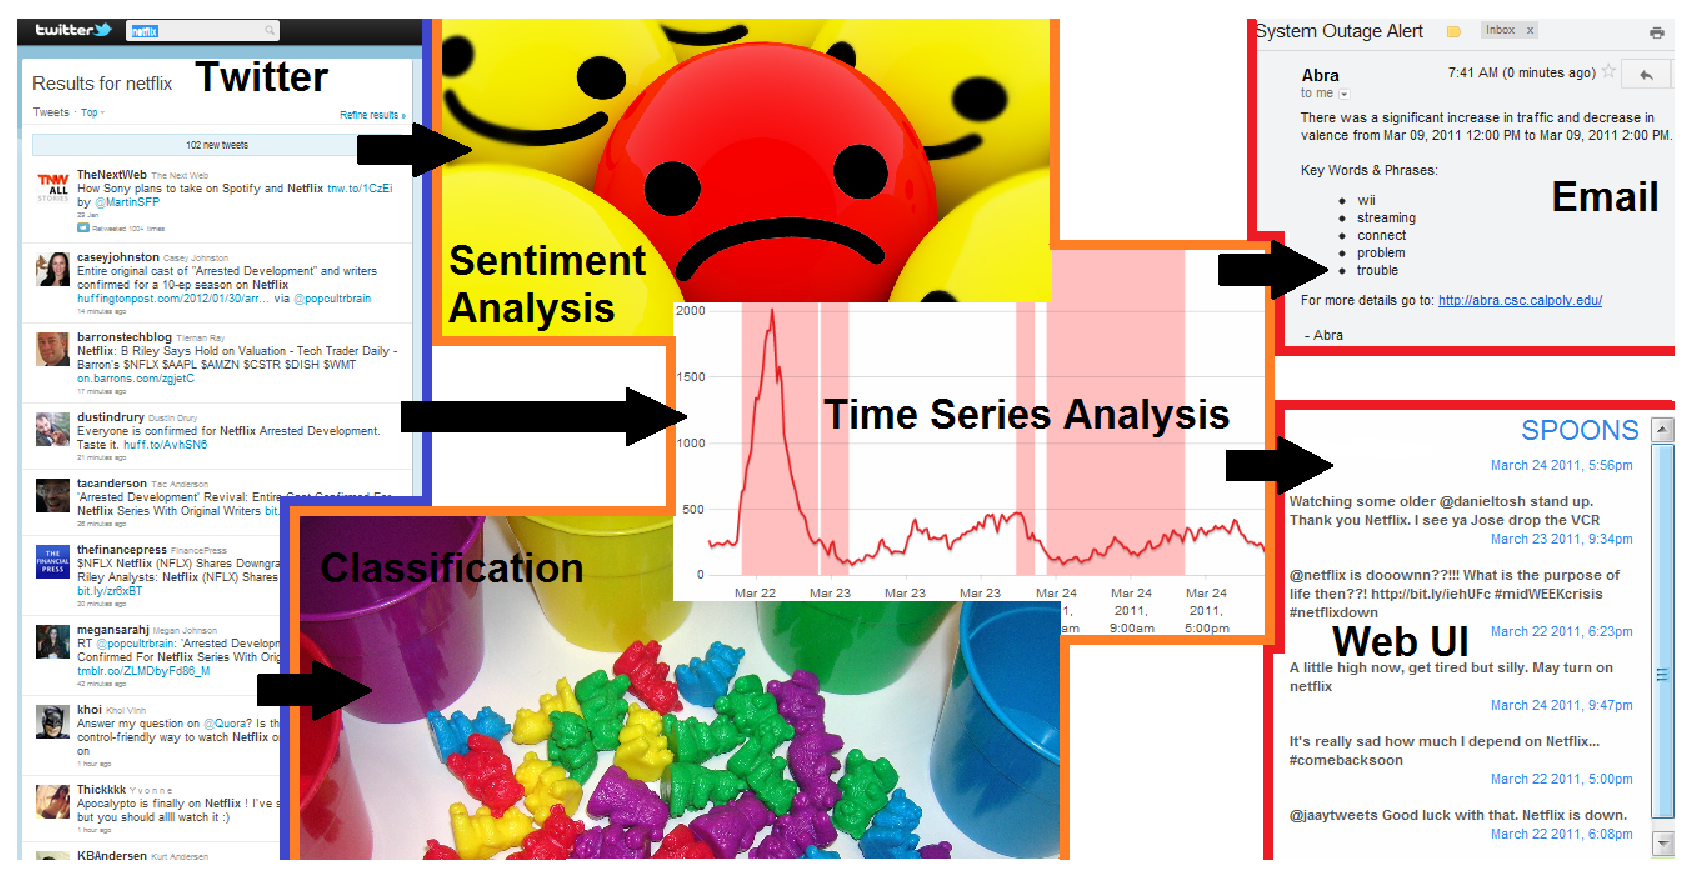
\includegraphics[width=140mm]{images/systemFlow.eps}
      \captionfonts
      \caption[System Concept Diagram]{This system concept diagram shows the general
                                       flow of processing done in the SPOONS system.}
      \label{fig:systemFlow}
   \end{center}
\end{figure}

Image~\ref{fig:systemFlow} shows how the SPOONS system can be divided into 3
main parts: {\color{blue}input}; {\color{orange}analysis methods}; and
{\color{red}output}. The inputs are tweets gathered from Twitter. Then the
analysis methods use a combination of sentiment estimation, classification, and
traffic volume analysis to detect when an outage is occurring.
The outputs of the system are: email alerts to Netflix engineers; and a web UI that displays
information about the outage.

\section{Ethics of Twitter Observation}

The work in this project uses content that people post on Twitter without their
knowledge. This monitoring system isn't being announced to the
public because wide spread knowledge of it would increase the likelyhood of a
malicious attack. This practice may lead to concerns about the level of privacy
or ownership being provided to Twitter users regarding the content they post
through the Twitter services. The goal of this section is to address these
concerns by proving more information about the Twitter services and how the
SPOONS system and this work uses the tweets.

\subsection{Twitter Terms of Service}

According to Twitter Terms of Service\cite{termsOfService} agreement, that
everyone accepts automatically by accessing or using Twitter services:

\emph{``You retain your rights to any Content you submit, post or
display on or through the Services. By submitting, posting or displaying Content
on or through the Services, you grant us a worldwide, non-exclusive,
royalty-free license (with the right to sublicense) to use, copy, reproduce,
process, adapt, modify, publish, transmit, display and distribute such Content
in any and all media or distribution methods (now known or later developed).''}

\emph{``This license is you authorizing us to make your Tweets available to the
rest of the world and to let others do the same.''}

\emph{``You agree that this license includes the right for Twitter to make such
Content available to other companies, organizations or individuals who partner with
Twitter for the syndication, broadcast, distribution or publication of such
Content on other media and services, subject to our terms and conditions for
such Content use.''}

\emph{``We encourage and permit broad re-use of Content. The Twitter API exists to
enable this.''}

\emph{``Such additional uses by Twitter, or other companies, organizations or
individuals who partner with Twitter, may be made with no compensation paid to
you with respect to the Content that you submit, post, transmit or otherwise
make available through the Services.''}

To summarize, while Twitter users do own the content they post,
by posting it through a Twitter service, they give Twitter and its partners
rights to reuse it without compensation. As a user of the Twitter API, the
SPOONS research group has become a partner of Twitter. So the analysis of
tweets, extraction of tweet metadata, and aggregate use of that data is well
within the rights of a partner of Twitter as defined by the Twitter Terms of
Service.

\section{SPOONS Requirements}
Netflix has provided the following set of key requirements to be met by the
SPOONS system:

\paragraph{Structural Independence}
The outage detection system shall be structurally independent of both the
software and the hardware infrastructure used by Netflix. It shall rely only on
information that is publicly available and free for use. This ensures that the
outage detection system stays up even when any or all Netflix servers are
experiencing downtime.

\paragraph{Use of Amazon Web Services}
Netflix is one of the largest customers of Amazon.com's cloud computing
service, Amazon Web Services (AWS). AWS allows users to create new cloud
machines (instances) in many regions throughout the world. The outage
detection system shall be deployed on one or more AWS servers that are
operationally independent of other AWS servers used by Netflix. Using a cloud
solution allows the outage detection and alert system to be deployable on a
global scale.

\paragraph{Real-Time}
Netflix's streaming services run in real-time and any downtime has an immediate
impact on customers. To minimize that impact, the outage detection system shall notify
Netflix of detected outages as soon as possible.

\paragraph{Precise Outage Detection}
The number of non-outage situations that raise an alert shall be minimized.
While a small number of false positives detected in real-time may be acceptable,
the outage detection system shall detect outages and generate alerts with as
high precision as possible.

\paragraph{Comprehensive Outage Detection}
Not all Netflix outages will generate a signal on Twitter. Those that don't may
be allowed to go unnoticed by the outage detection system (as the system will
have no basis for detecting them), but any outage that causes a signal on
Twitter shall be detected.

\paragraph{User-Friendly Online UI}
The outage detection and alert system shall have an easy-to-use, informative,
online UI which shall provide Netflix employees with real-time information and
historic data about the state of Netflix according to Twitter. The information
provided shall include:

\begin{itemize}
   \item times of outages;
   \item times of other anomalous events;
   \item current and recent Netflix-related Twitter traffic trends;
   \item and samples of Netflix-related tweets.
\end{itemize}

\chapter{Background \& Related Work}
\label{background-related-work}

\section{Text Stream Analysis}
\label{background-text-stream}
Text Stream Analysis \cite{Bansal}\cite{Grinev}\cite{Huang}.

\section{Classification}
\label{background-classification}
Classification \cite{Pang}

\subsection{Microtext Classification}
\label{background-microtext-classification}
Microtext Classification \cite{hong}

\subsection{WEKA}
\label{background-weka}
\begin{wrapfigure}{r}{0.20\textwidth}
  \begin{center}
    
\includegraphics[width=0.20\textwidth]{images/weka.eps}
  \end{center}
  \caption{WEKA logo}
\end{wrapfigure}
SPOONS utilizes several classifiers provided in the WEKA machine learning package.
WEKA is an open source package written under the GNU General Public License\cite{weka}.

\section{Twitter API}
\label{background-twitter-api}
All of the data data that SPOONS uses is obtained in real time using the Twitter Search REST API\cite{TwitterAPI}.

\subsection{Rate Limiting}
\label{api-rate-limit}
Twitter imposes a limit on the number of queries to the Search API. However, Twitter does not publish the official
limit. However, my experiments suggests that SPOONS can query the API for all new Tweets once every two minutes without
suffering from rate limiting.

\subsection{Pagination}
\label{api-pagination}
Twitter paginates the results from its search api. The maximum results you can get per page is 100, and each
query can return at most 15 pages. Therefore when there are more than 1500 tweets generated per minute,
SPOONS must do multiple seach queries.

\subsection{Query Anatomy}
\label{api-anatomy}
One of our typical queries looks like:\\
http://search.twitter.com/search.\textbf{json}?\textbf{q}=$\langle$query$\rangle$\&\textbf{rpp}=100\&\textbf{result\_type}=recent\&\textbf{since\_id}=$\langle$tweet id$\rangle$\&\textbf{max\_id}=$\langle$tweet id$\rangle$

\paragraph{json}
Twitter can supply the result data in either ATOM or JSON format. Testing with both have shown that the ATOM
results are less consistent and provide less data. Because of the more accutate information returned from the JSON
api, we are able to write more efficient queries. Using the ATOM api, we could query Twitter only once every five
minutes; as opposed to every two minutes with the JSON api.

\paragraph{q}
The search query. Twitter supports some advanced search features such as conjunction and negation.

\paragraph{rpp}
``Results Per Page''. Twitter paginates the responses from the Search API. SPOONS always uses the maximum pagination value to decrease the number of requests per hour and lessen the change of being rate limited.

\paragraph{result\_type}
Twitter allows users to get results orderd search by either relevance or time. Since we want to gather all tweets about
our query, we choose to get the results ordered by time. In addition, the ``since\_id'' and ``max\_id''
parameters do not work when results are sorted by relevance.

\paragraph{since\_id}
The id of the oldest tweet that should be returned. This is not a hard limit, but provides a nice starting point.

\paragraph{max\_id}
The id of the most recent tweet that should be returned. It may seem counter-intuitive to provide a cap on the
most recent tweet, when one wants to query for all of the most recent tweets. However when a query spans across
more than 15 pages, it will need to be broken into a new query restarting at the first page. In this situation,
not providing an upper limit will include new tweets outside of the original search scope. This can result in tweets
are forever lost to us.

\subsection{Result Anatomy}
\begin{figure}
   \begin{center}
      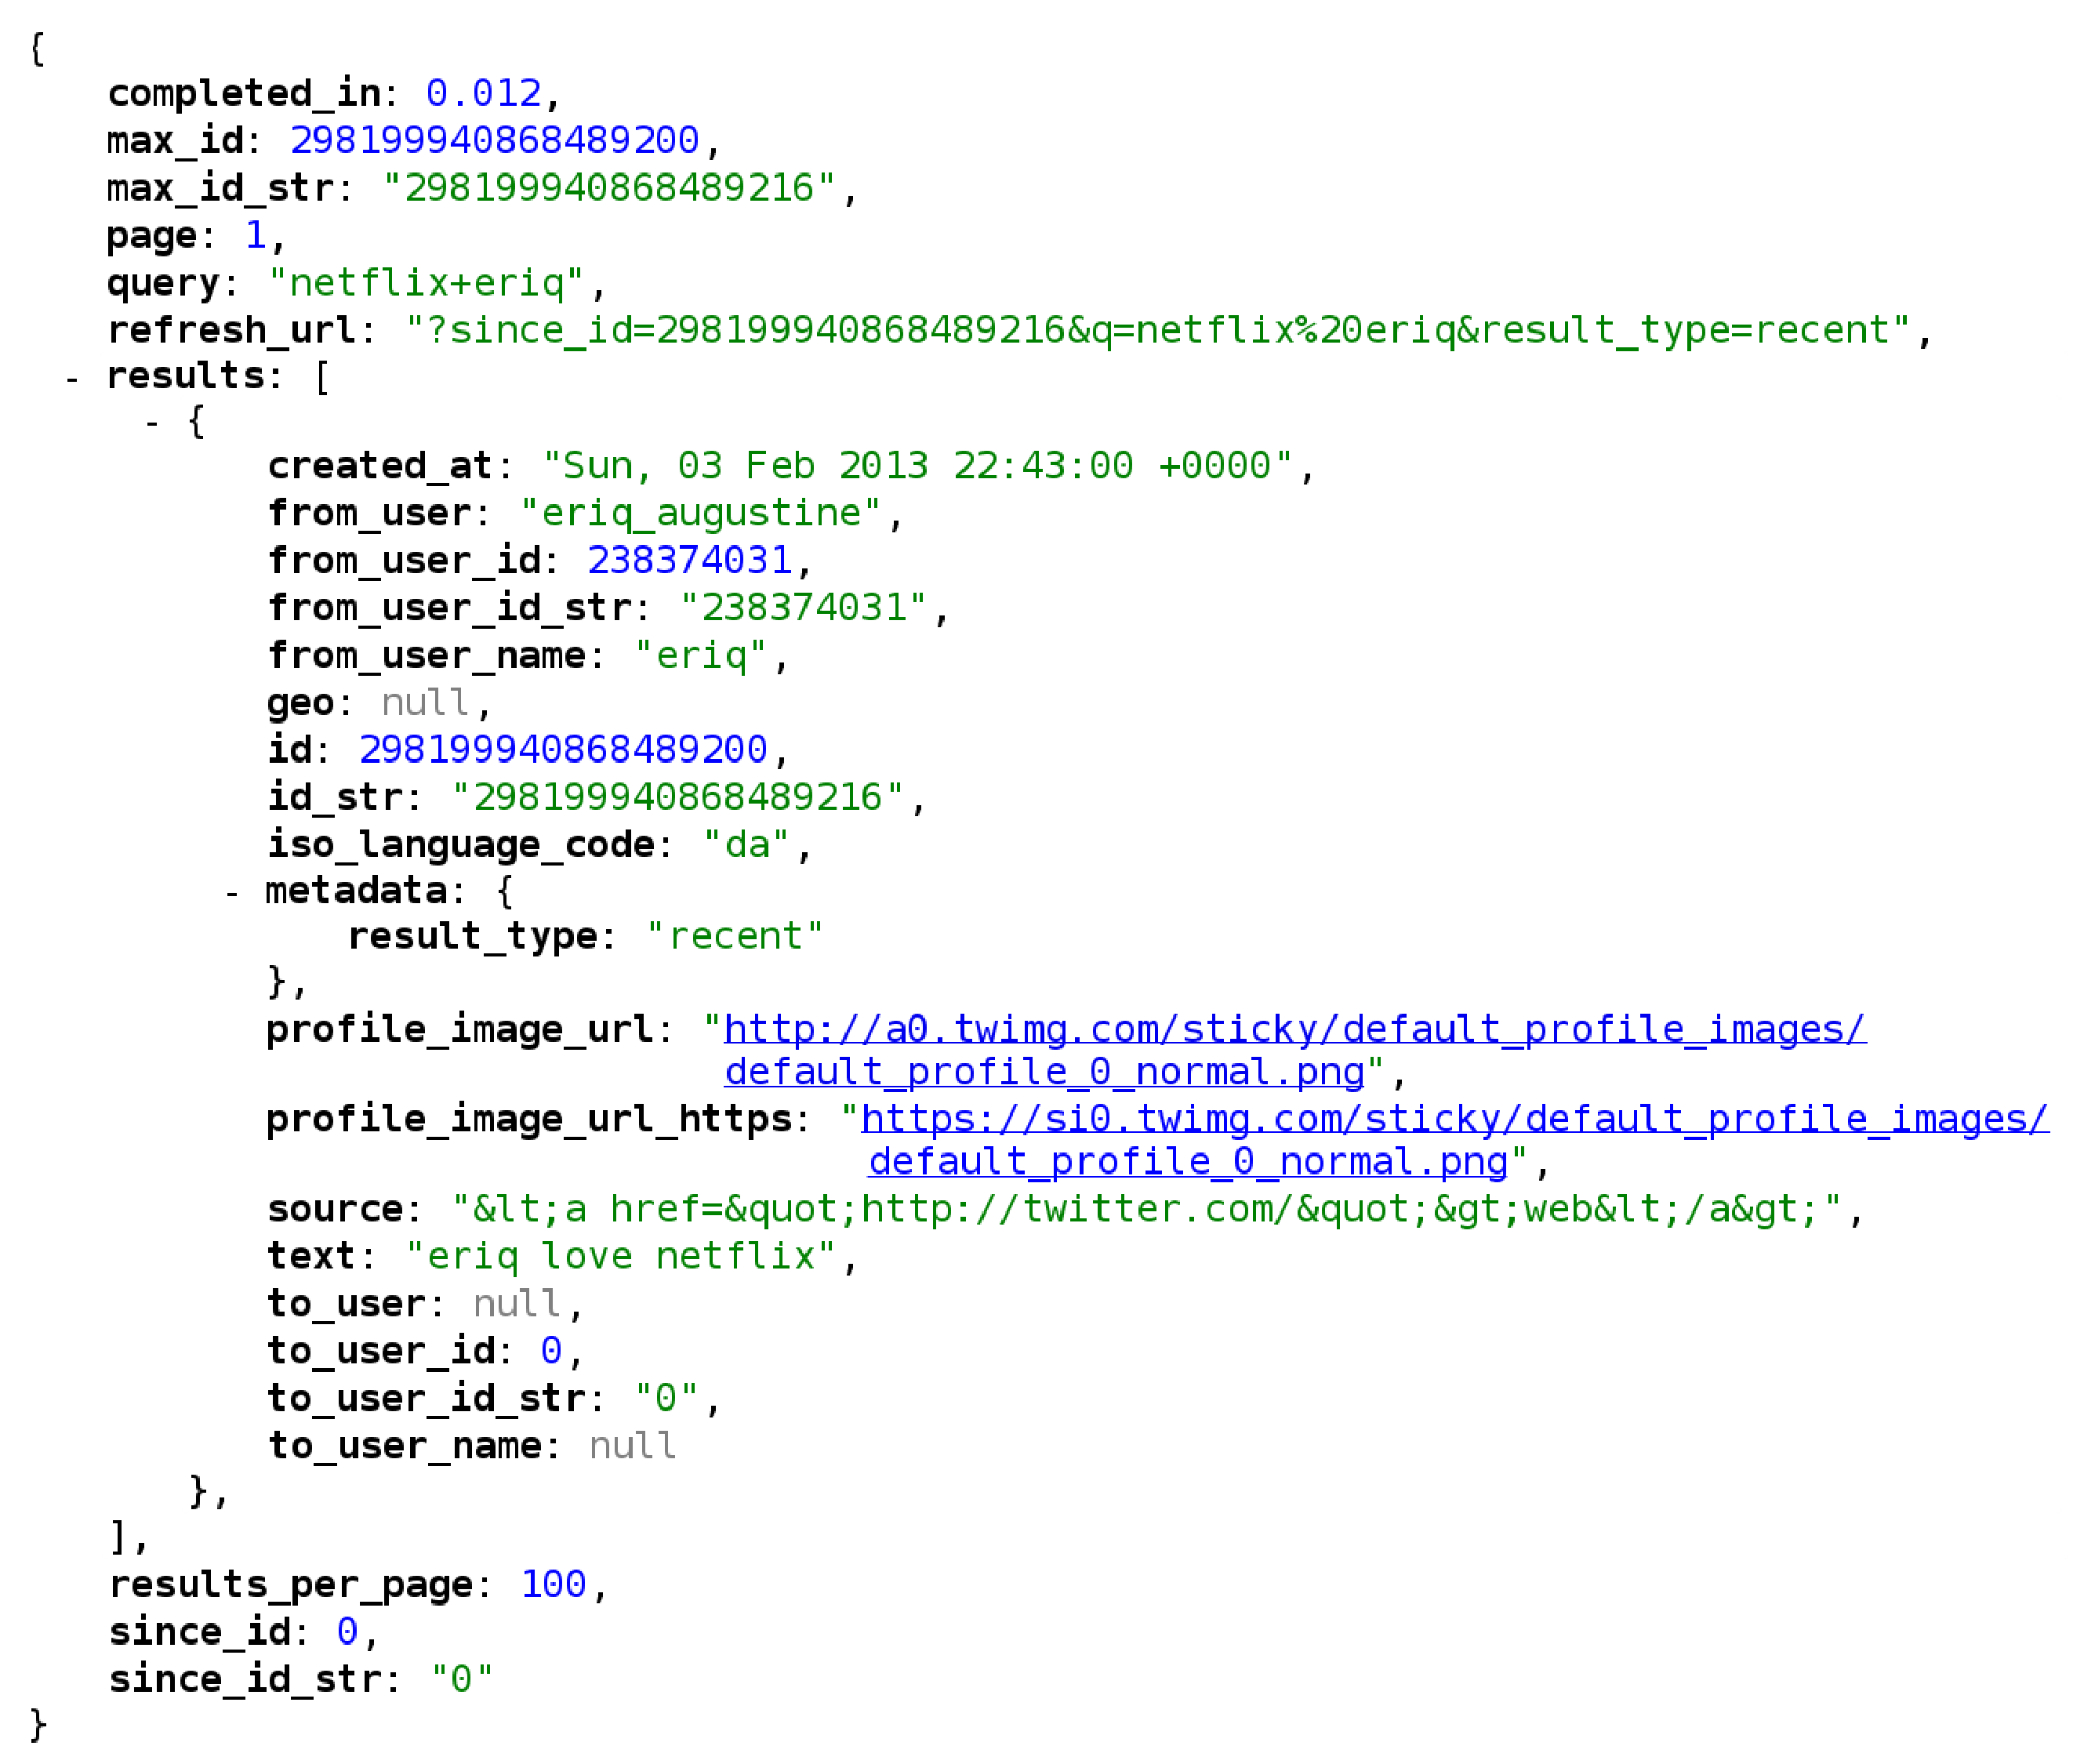
\includegraphics[width=140mm]{images/api_result.eps}
      \captionfonts
      \caption[Twitter Search API Result]{A JSON result from the Twitter Search API}
      \label{fig:apiRes}
   \end{center}
\end{figure}

Image~\ref{fig:apiRes} shows the result from the query ``eriq netflix''. Notice that some fields,
like the ``geo'' field, can be null. Also note that the api incorrectly guessed my language as Danish.

\chapter{SPOONS Architecture}
\label{arch}

\section{Architecture Overview}
\label{arch-overview}
\begin{figure}
   \begin{center}
      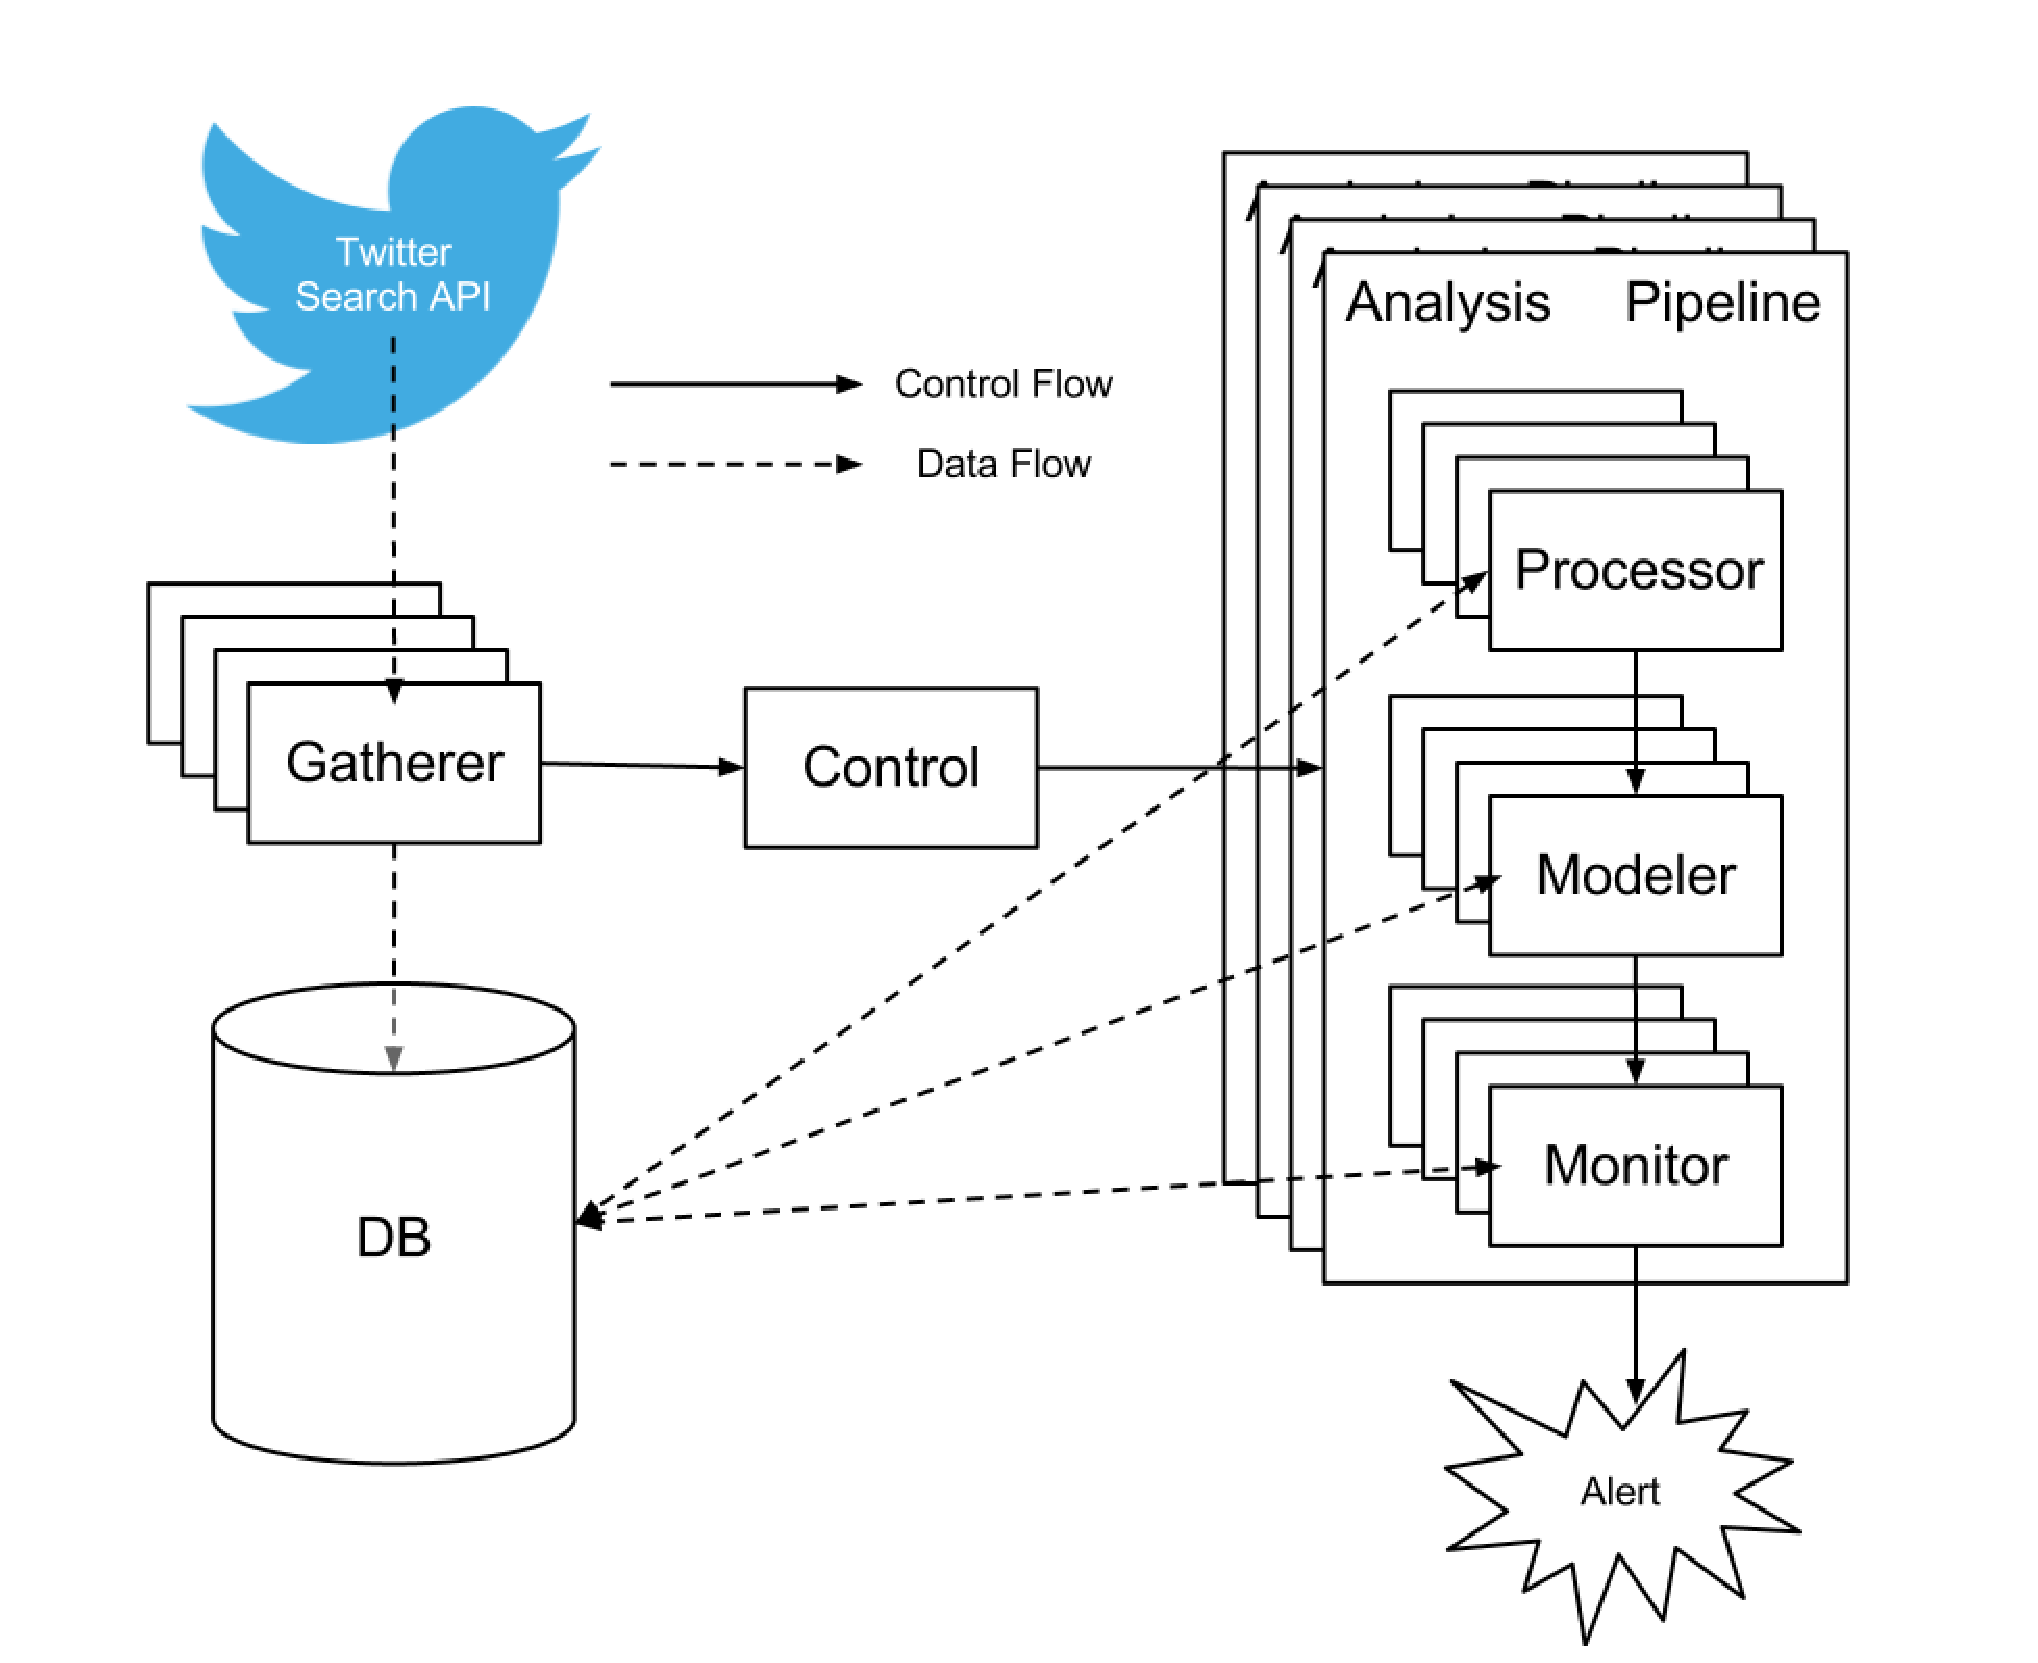
\includegraphics[width=0.8\textwidth]{images/SPOONS_Framework_Architecture.eps}
      \captionfonts
      \caption[SPOONS Framework Architecture]{The flow of control and data through the SPOONS framework system.}
      \label{fig:frameworkArch}
   \end{center}
\end{figure}

There are multiple levels of architecture within SPOONS that need to be discused.
There is the Framework Architecture (Image~\ref{fig:frameworkArch}) that describes the relations between the
different pieces of the framework; the Server Architecture (Image~\ref{fig:serverArch}) that describes the layout of
the different servers involved in the SPOONS system; and the Distribution Model which describes how tasks are
distributed between the different servers.

\subsection{Claims}
\label{arch-claims}
As part of my thesis, I lay claim to the design and implementation of the SPOONS system, framework, server architecture,
distribution model, and database schema. However, I do not claim the UI and API. Those were the product of Matt Tognetti.

\subsection{Backend}
\label{arch-backend}
The ``backend'' consists of all parts of SPOONS that are not part of the UI or API.
This includes code that runs on multiple servers as well as the database.

\subsection{UI and API}
\label{arch-ui}
\begin{figure}
   \begin{center}
      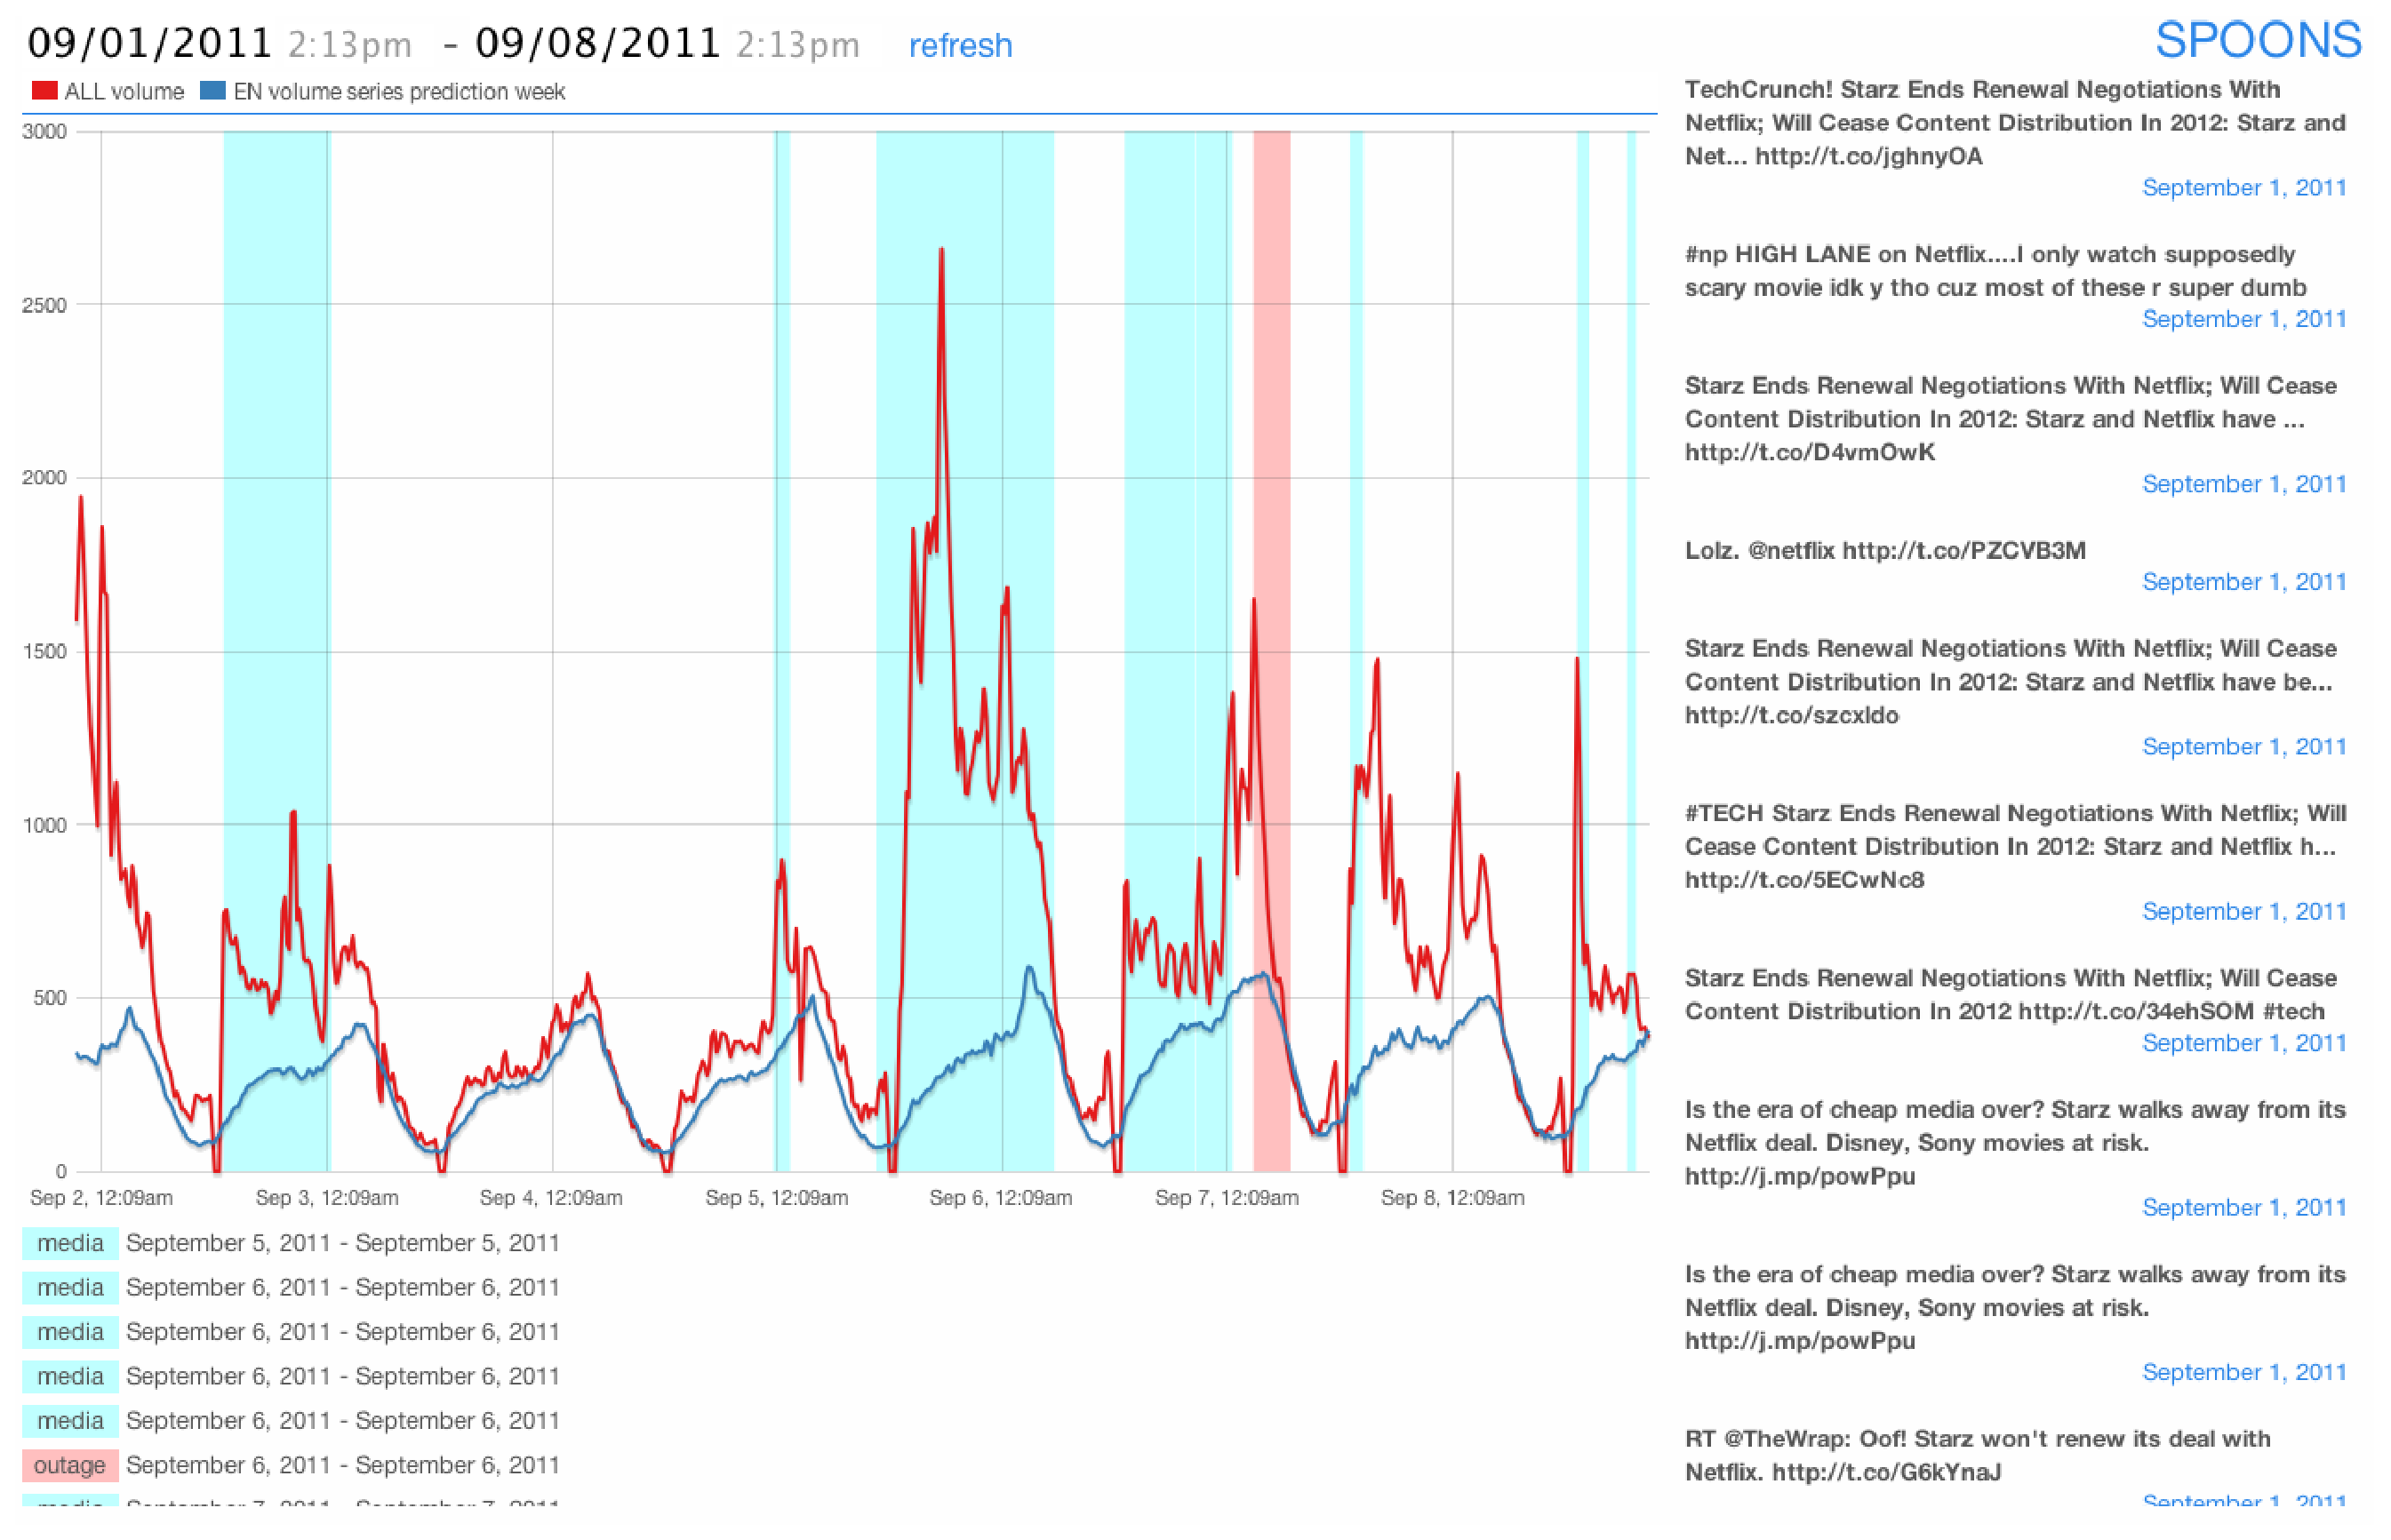
\includegraphics[width=0.8\textwidth]{images/ui.eps}
      \captionfonts
      \caption[SPOONS UI]{The web UI for SPOONS.}
      \label{fig:ui}
   \end{center}
\end{figure}

SPOONS includs a web UI that allows users to quickly and easily view the data produced by SPOONS.
The UI is written primarily in PHP and Javascript and is seperated from the SPOONS backend.
The only shared resource between the UI and backend is the database. The UI will automatically pull
data from tables that have a specified schema and present them to the user.

\section{Framework Architecture}
\label{arch-framework-arch}
This section describes the architecture of the SPOONS framework. The SPOONS framework includes all pieces of SPOONS
that takes the data from gathering all the way through to final analysis.

\subsection{Gatherers}
\label{arch-gatherers}
The data begins its journey in the Gatherers. The Gatherers run periodically (for Twitter, every two minutes).
Gatherers are asynchronous and not dependent on any other part of the framework. There may be multiple different
Gatherers running on the same machine. Gatherers are abstracted to be able to gather data from any source.
Once the Gatherers get their data, they place the data in the database and notify the Control that there is new data
available to the system.

\subsubsection{Twitter Holes}
\label{arch-twitter-holes}
It is worth noting that sometimes the Twitter Search API fails to return any data. We have not discovered the cause
of this, but Twitter does not report any errors. For unspecified amounts of time the Twitter API will just report zero
new tweets. We call these dead zones ``holes''. We have found that a query from a different IP usaully does not
experience the same hole. To counteract holes, we run Gatherers on multiple servers and resolve uniques upon insertion
into the database.

\subsection{Processors}
\label{arch-processors}
Processors are responsible for processing or transforming data before it goes into the analysis pipelines.
Processing the data could be any task. Some of our most notable Processors are ones that classifies tweets into one of
the nine tweet categories discussed in Section~\ref{class-tweet-classes}.

Unlike most parts of the analysis pipeline, Processors are a shared resource. That is, multiple analysis pipelines
invokle the same processors. However, it does not make sense to restart the processing once it is started, or to
start another instance of the same Processor. Processors have a finite amount of data to process and may be cumulative.
Therefore, Processors are singleton. When multiple threads call into a Processor to do work, the Processor will block
all incoming threads until the work is complete. Then, the Processor will release all of the threads that asked it to
do work. This model allows all the analysis pipelines to share the same Processor without any duplication of work.

\subsection{Analysis Pipelines}
\label{arch-pipelines}
An Analysis Pipeline (also called Analysis Method) is the analytical center of the SPOONS framework.
The pipeline aggregates multiple tasks that it needs to run on the data.

An Analysis Pipeline typically starts with running any number of processors on the data.
Then, the pipeline invokes modelers on the data from the Processors. These modelers typically build models and
predictive models on the data. Finally, the pipeline invokes tasks that asses the models produced in the previous
step and decides whether or not there is an anomaly.

Every Analysis Pipeline gets its own thread, and there is no interdependence between the different pipelines.
Currently, SPOONS usually runs more than 20 Analysis Pipelines at a time.

\subsubsection{Tasks}
\label{arch-tasks}
Tasks are the core unit of computation in SPOONS. Almost everything that can be ``run'' is a child of the Task base
class. Every Task gets its own thread, and callers into the Task may request that the task block the calling thread
until the Task is complete.

Tasks are singleton with respects to the leaf child class. Therefore there are many tasks, but every task is
unique. We do this by enforcing that the class name is unique upon construction. The uniqueness of tasks is very
important to SPOONS distribution model that will be discussed in Section~\ref{arch-dist}.

\subsubsection{Modelers}
\label{arch-modelers}
Modelers are Tasks that are responsible for building a mathematical representation for the data.

\paragraph{Predictors}
\label{arch-predictors}
Predictors build a predictive model of the data. For example, we have noticed that tweet volume tends to be
periodic day-to-day and week-to-week. Therefore, a Predictor may just model that prediction by guessing that the volume
in the future will be the same as it was the previous week or day.

\paragraph{Counters}
\label{arch-counters}
Counters attempt to build a model of data that was actually gathered by the system. Going with the previous example,
the Counter for modeling tweet volume would simple count the number of tweets gathered for a period.

\subsubsection{Monitors}
\label{arch-monitors}
Monitors take the models produced by the Predictors and Counters and compares them. The Monitors are responsible for
making the final decision on about a period of time being anomalous.

\paragraph{Auto-Tuning}
\label{arch-autotuning}

\subsection{Control}
\label{arch-control}

\subsubsection{Master Control}
\label{arch-master-control}

\subsubsection{Worker Control}
\label{arch-worker-control}

\subsubsection{Single Control}
\label{arch-single-control}

\subsection{Distributed Model}
\label{arch-dist}

\subsubsection{Distributable Tasks}
\label{arch-tasks}

\begin{figure}
   \begin{center}
      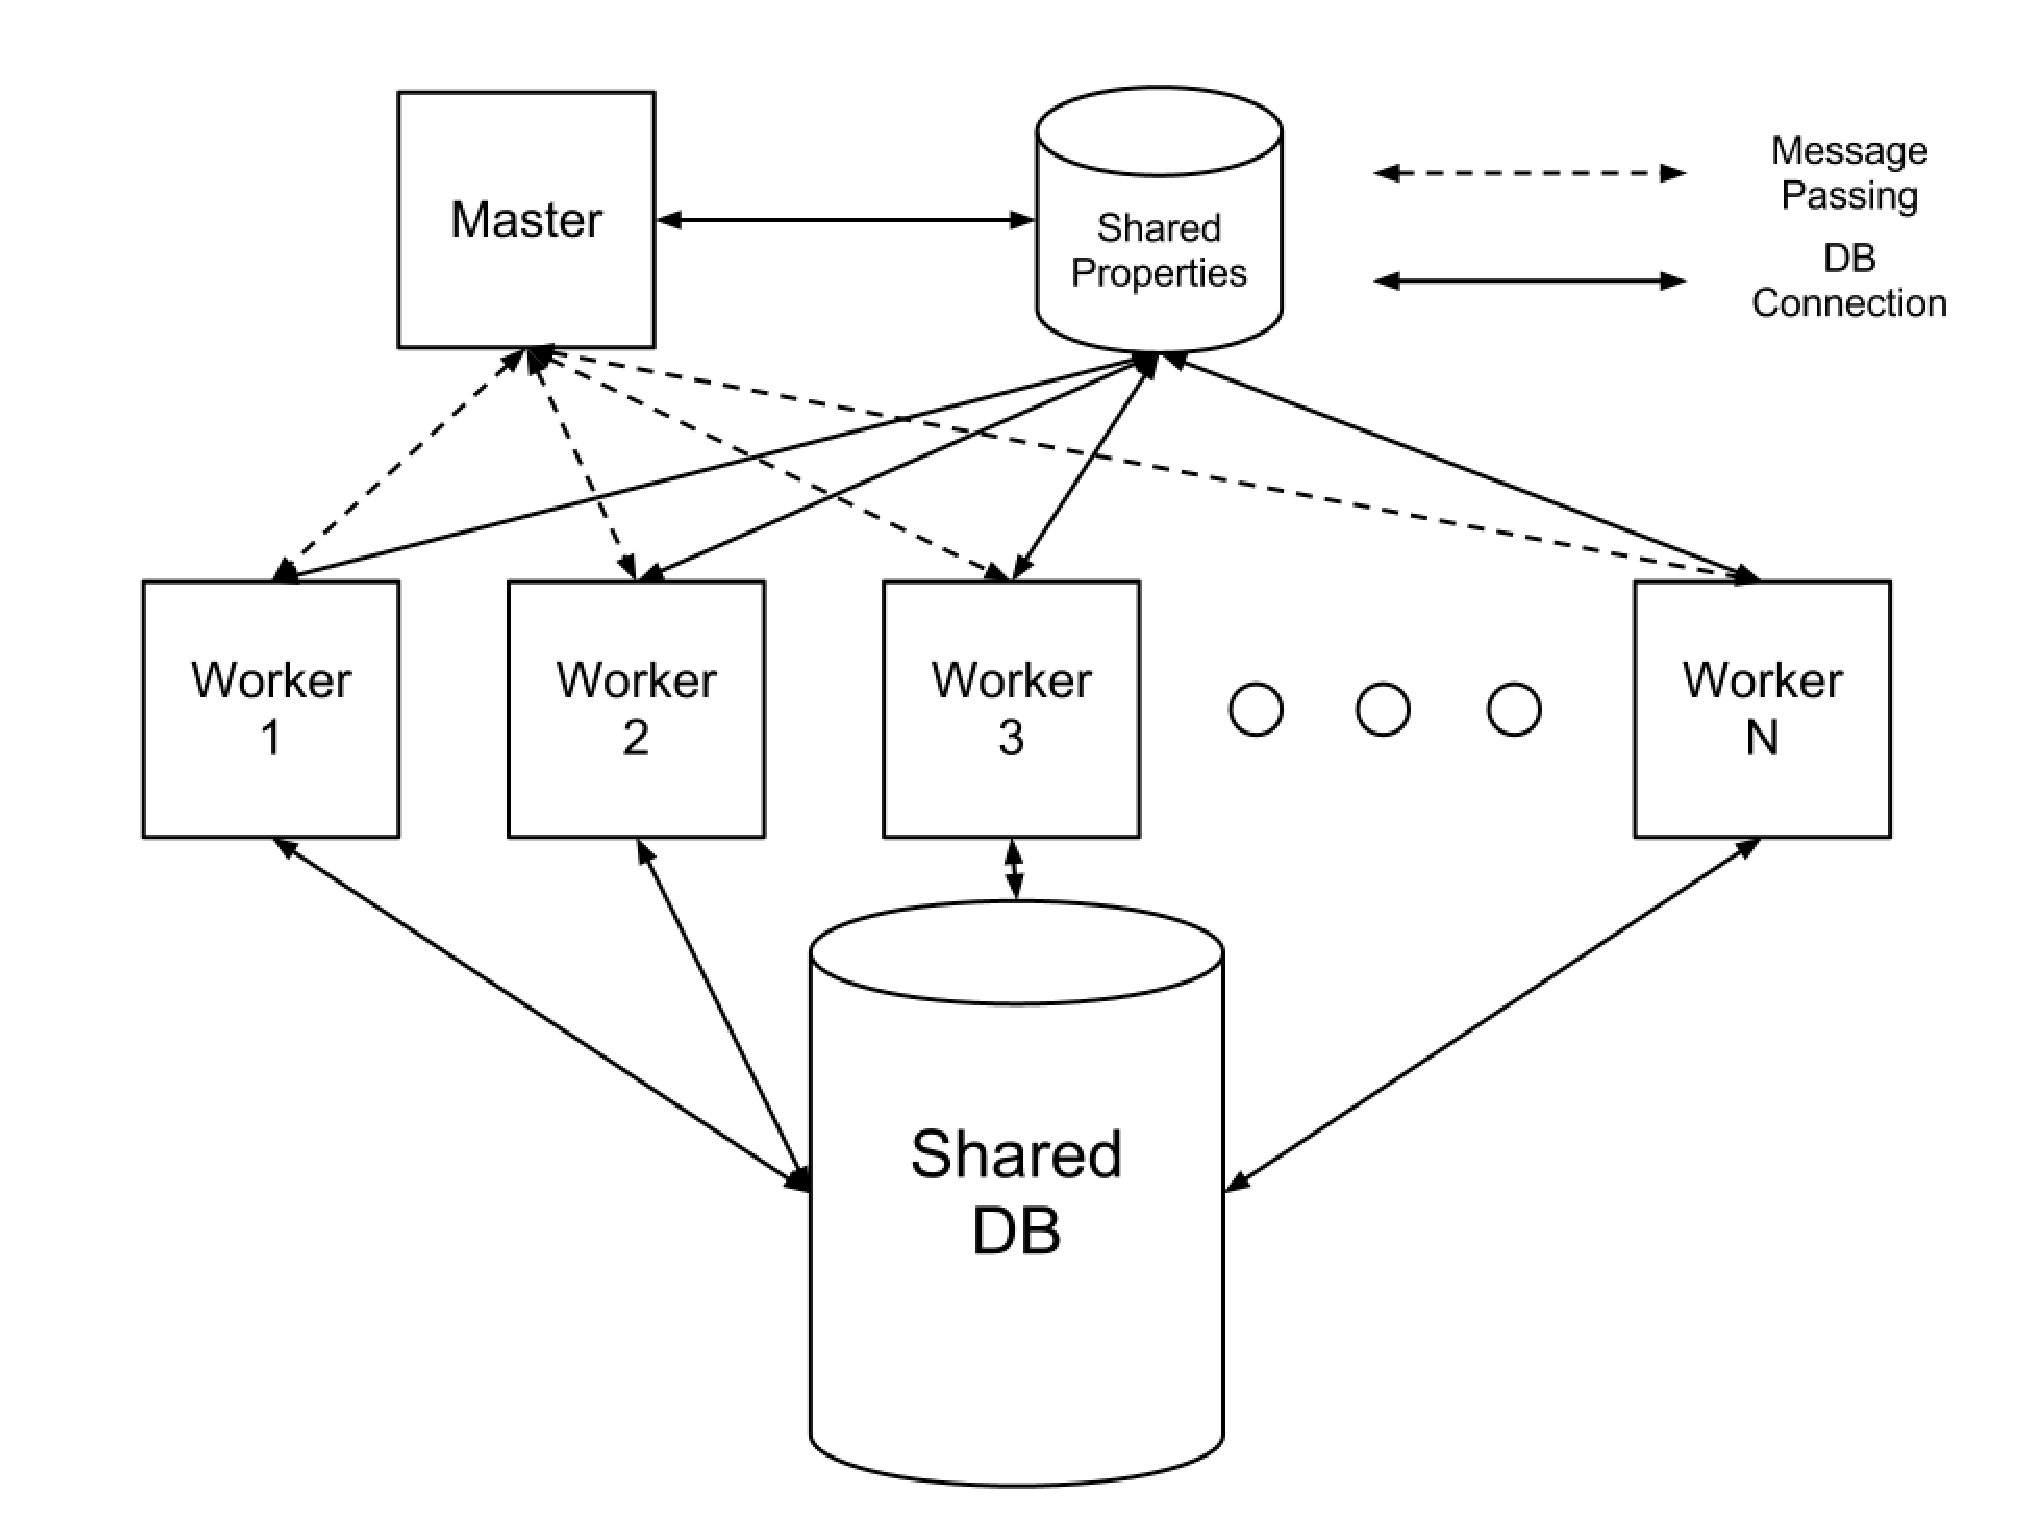
\includegraphics[width=0.8\textwidth]{images/SPOONS_Server_Architecture.eps}
      \captionfonts
      \caption[SPOONS Server Architecture]{The server architecture of the SPOONS system.}
      \label{fig:serverArch}
   \end{center}
\end{figure}

\begin{figure}
   \begin{center}
      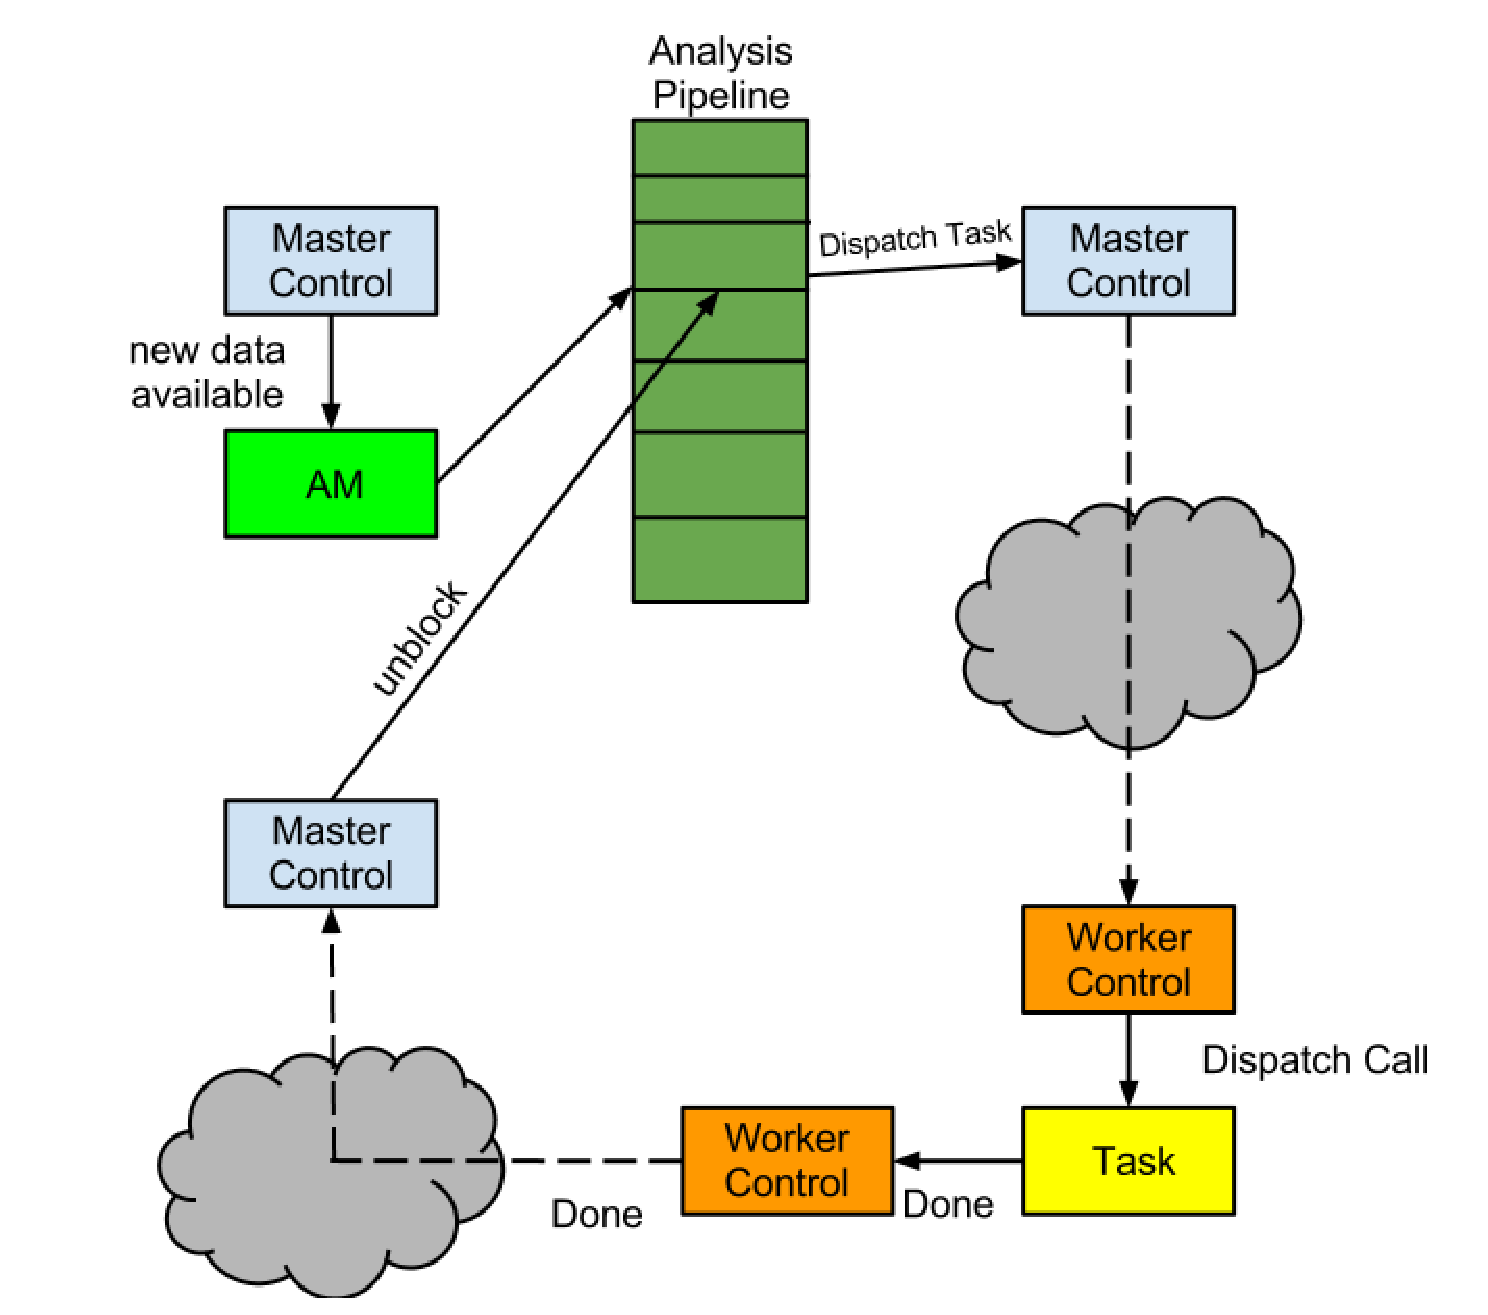
\includegraphics[width=0.8\textwidth]{images/SPOONS_Distributable_Task_Control_Flow.eps}
      \captionfonts
      \caption[SPOONS Distributable Task Flow]{The control flow for distributable tasks.}
      \label{fig:serverArch}
   \end{center}
\end{figure}

\section{Database}
\label{arch-database}

\subsection{Tables and Schemas}
\label{arch-database-tables}

\section{Analytical Framework}
\label{arch-framework}
How do you plug into the framework.
Instantiation based.

\chapter{Classifiers}
\label{classifiers}

\section{Fitting Into The SPOONS Framework}
\label{class-framework}

\section{WEKA Classifiers}
\label{class-weka}

\section{Non-WEKA Classifiers}
\label{class-nonweka}

\section{Feature Selection}
\label{class-features}

\subsection{Text Filtering}
\label{class-filtering}

\subsubsection{Twitter Specific Symbols}
\label{class-twitter-symbols}

\subsubsection{Emoticon Parsing}
\label{class-emoticon}

\subsubsection{Title Replacement}
\label{class-title}

\subsubsection{Stemming}
\label{class-stemming}
Perhaps not a ful subsubsection for this, just Porters

\subsubsection{Stop Word Removal}
\label{class-stopword}

\section{Tweet Classes}
\label{class-tweet-classes}

\subsection{Tweet Groups}
\label{class-tweet-groups}

\section{Training Set}
\label{class-training-set}

\chapter{Experimental Setup}
\label{experiments}

\section{Ground Truth}
\label{exp-truth}

\section{Success Metrics}
\label{exp-metrics}

\section{Classifier Evaluation}
\label{exp-classifier}

\section{Outage Detection}
\label{exp-outage}

\subsection{Monitor Parameters}
\label{exp-monitor-params}

\chapter{Results}
\label{results}

\section{Classifier Evaluation}
\label{res-classifier}

\section{Outage Detection}
\label{res-outage}

\chapter{Conclusions}
\label{conclusions}

\section{Current Limitations of SPOONS}
\label{limitations}
Severity
Nature of Outage
Malicious Tweet Attack
Know What To Search For (dynamic search generation)

\section{Current and Future Work}
\label{future-work}
Kim - Advanced Sentiment Analysis
Brett - Feasability of SPOONS as a comercial multi-target, source system.
All sorts of stuff
Open Source System
Dynamic Training Set

% ------------- End main chapters ----------------------

% Glossary here plz
\newglossaryentry{SPOONS}{name={SPOONS},
                          description={Swift Perception Of Online Negative Situations. The name
                                       of the system presented in this paper}}

\newglossaryentry{Twitter}{name={Twitter},
                           description={Twitter is a social media service that allows users to post
                                        tweets (micro-posts) about any topic}}

\newglossaryentry{Tweet}{name={Tweet},
                         description={A micro-post to a Twitter service. Tweets are limited to 140
                                      characters}}

\newglossaryentry{Netflix}{name={Netflix},
                           description={Inc. [NASDAQ: NFLX] is the world's leading Internet
                                        subscription service for enjoying movies and TV series
                                        with more than 23 million streaming members in the United
                                        States, Canada, Latin America, the United Kingdom
                                        and Ireland\cite{netflix}}}

\newglossaryentry{Time Series Analysis}
      {name={Time Series Analysis},
       description={The analysis of a series of data points over time. In this work those data
                    points are the volume or estimated sentiment of a subset of the traffic about
                    Netflix on Twitter during a time period}}

\newglossaryentry{Real Time}
      {name={Real Time},
       description={Some of Netflix's services stream to customers in real time which means the
                    users expect to get immediate responses from those services. So when
                    they go down, the customers want the problem to be fixed immediately. These
                    analysis methods need to have real time responses that are as close to
                    immediate detection as possible. This means that the system needs to use
                    whatever information it has available to it up to right before the outage to
                    detect the event and alert Netflix engineers}}

\newglossaryentry{aws}
      {name={AWS},
       description={Amazon Web Services. Cloud computing offerd by Amazon}}

\newglossaryentry{ec2}
      {name={EC2},
       description={Elastic Compute Cloud. Instance based cloud computing machines offered through AWS}}

\glsaddall
\addcontentsline{toc}{chapter}{Glossary}
\printglossaries

\clearpage
\bibliography{bibliography}
\bibliographystyle{plain}
%\addcontentsline{toc}{chapter}{Bibliography}

\end{document}
